\documentclass[11pt]{article}
\usepackage[a4paper,left=1.5cm,right=1.5cm,top=1.5cm,bottom=1.5cm]{geometry}
\usepackage{fancyhdr}
\renewcommand{\headrulewidth}{1pt}
\fancyhead[C]{\textbf{[LINMA1170] Solveurs itératifs}}
\fancyhead[L]{Décembre 2018}
\fancyhead[R]{Gilles Peiffer [24321600]}

\usepackage[T1]{fontenc}
\usepackage[utf8]{inputenc}
\usepackage[french]{babel}
\usepackage{graphicx}
\usepackage{subcaption}
\usepackage{csquotes}
\usepackage{mathtools,amssymb}
\usepackage[binary-units=true,separate-uncertainty = true,multi-part-units=single]{siunitx}
\usepackage{float}
\usepackage[linktoc=all]{hyperref}
\hypersetup{breaklinks=true}
\setlength{\parskip}{1ex plus 0.5ex minus 0.2ex}
\newcommand{\hsp}{\hspace{20pt}}
\newcommand{\HRule}{\rule{\linewidth}{0.5mm}}
\graphicspath{{img/}}
\usepackage{caption}
\usepackage{textcomp}
\usepackage{array}
\usepackage{color}
\usepackage{tabularx,booktabs}
\usepackage{titlesec}
\usepackage{wrapfig}
\titlespacing{\section}{0pt}{\parskip}{-\parskip}
\titlespacing{\subsection}{0pt}{\parskip}{-\parskip}
\titlespacing{\subsubsection}{0pt}{\parskip}{-\parskip}
\pagestyle{fancy}
\DeclarePairedDelimiterX{\norm}[1]{\lVert}{\rVert}{#1}
\newcommand{\abs}[1]{\left\lvert#1\right\lvert}
\usepackage{listings}
\lstset{
	language=Python,
	numbers=left,
	numberstyle=\tiny\color{gray},
	basicstyle=\rm\small\ttfamily,
	keywordstyle=\bfseries\color{dkred},
	frame=single,
	commentstyle=\color{gray}=small,
	stringstyle=\color{dkgreen},
	%backgroundcolor=\color{gray!10},
	%tabsize=8, % Thank you Papa Torvalds
	%rulecolor=\color{black!30},
	%title=\lstname,
	breaklines=true,
	framextopmargin=2pt,
	framexbottommargin=2pt,
	extendedchars=true,
	inputencoding=utf8,
}
\DeclareMathOperator{\dens}{\mathrm{dens}}

\begin{document}
\section*{Introduction}
Pour ce devoir, il était demandé d'écrire des fonctions en langage Python permettant de résoudre éfficacement un système d'équations linéaires issu d'un modèle d'éléments finis appelé \lstinline[language=bash]{ccore} en utilisant un algorithme de gradients conjugués. La résolution est donc faite de façon itérative, et l'influence du préconditionneur \texttt{ILU0} est également montrée. Une attention particulière est apportée à l'étude de l'évolution du conditionnement de la matrice d'éléments finis, facteur très important pour la vitesse de convergence du solveur.

\section{Effet du préconditionneur}
\label{sec:prec}
Pour la première question, il était demandé d'observer l'effet du préconditionnement sur le conditionnement de la matrice, ainsi que sur le spectre des valeurs propres de celle-ci.
On appelle $A \in \mathbb{C}^{n \times n}$ la matrice initiale, et $M \in \mathbb{C}^{n \times n}$ le préconditionneur \texttt{ILU0} utilisé.
Le systère que l'on résout devient alors $M^{-1} A x = M^{-1}b$ au lieu de $Ax = b$.
Le nombre d'itérations nécessaires pour une tolérance donné pour la méthode des gradients conjugués évolue en $\mathcal{O}\big(\sqrt{\kappa}\big)$, où $\kappa$ dénote le conditionnement de la matrice utilisée (soit $A$, soit $M^{-1}A$).
L'algorithme \texttt{ILU0} va calculer la matrice $M$ telle que $\kappa(M^{-1}A) \ll \kappa(A)$ et $\norm{M^{-1}A - I} \approx 0$.
On peut voir dans le livre de référence\footnote{Trefethen, Lloyd N. \& Bau, David \textrm{III}. (1997). \textit{Numerical Linear Algebra}. Philadelphia: \textsc{PA}, \textsc{SIAM}.} pp. 298--300 que les Théorèmes~38.3--5 affirment qu'afin de diminuer le nombre d'itérations nécessaires pour converger, nous pouvons jouer sur le spectre des valeurs propres de la matrice, $\Lambda$. En effet, un \foreignquote{french}{bon} spectre possède au moins l'une des deux qualités suivantes: ses valeurs propres sont fortement groupées et/ou son conditionnement $\kappa$ (le rapport $\abs{\lambda_{\max}} / \abs{\lambda_{\min}}$) est faible.
En affichant l'évolution du conditionnement de la matrice en fonction de l'évolution de l'un des trois paramètres (taille de l'entrefer, raffinement du maillage et perméabilité magnétique du noyau, chaque fois en fixant les deux autres), on observe que le conditionnement de la matrice préconditionnée est inférieur à celui de la matrice initiale pour les plages de valeurs choisies et les matrices issues du modèle \texttt{ccore}. Par souci de place, seul le graphe en fonction de la perméabilité relative est montré à la Figure~\ref{fig:mur_cond}, bien que le résultat soit similaire lorsque l'on joue sur les autres paramètres.

Regardons ensuite l'effet du préconditionnement sur le spectre des valeurs propres de la matrice. Comme dit ci-dessus, un \foreignquote{french}{bon} spectre est un spectre groupé. Afin d'observer ceci, il est intéressant de représenter le support du spectre, comme sur les graphes des Figures~\ref{fig:mur_spec} et \ref{fig:mur_spec_prec}. Comme les graphes sont semi-logarithmiques, il suffit de comparer les échelles des graphes pour voir que sur la Figure~\ref{fig:mur_spec_prec} les valeurs sont beaucoup mieux groupées et se trouvent beaucoup plus près de $1$, ce qui confirme que le conditionnement est bien plus faible pour la matrice préconditionnée dans le cas d'un changement de perméabilité relative aussi.

\begin{figure}[H]
	\centering
	\begin{subfigure}[t]{0.32\textwidth}
		\centering
		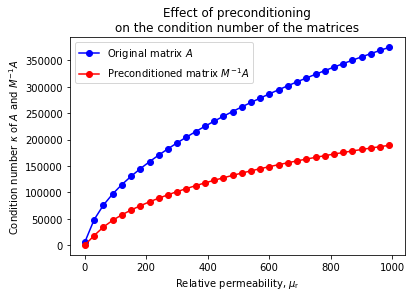
\includegraphics[width=\linewidth]{mur_cond.png}
		\caption{Évolution de $\kappa$ en fonction de la perméabilité relative pour une matrice avec et sans préconditionnement.}
		\label{fig:mur_cond}
	\end{subfigure}\hfill
	\begin{subfigure}[t]{0.32\textwidth}
		\centering
		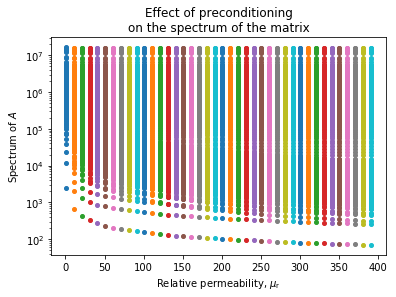
\includegraphics[width=\linewidth]{mur_spec.png}
		\caption{Évolution de $\Lambda$ en fonction de la perméabilité relative pour une matrice non préconditionnée.}
		\label{fig:mur_spec}
	\end{subfigure}\hfill
	\begin{subfigure}[t]{0.32\textwidth}
		\centering
		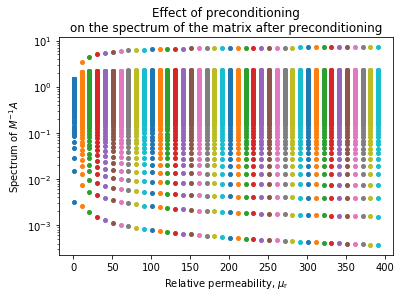
\includegraphics[width=\linewidth]{mur_spec_prec.png}
		\caption{Évolution de $\Lambda$ en fonction de la perméabilité relative pour une matrice préconditionnée.}
		\label{fig:mur_spec_prec}
	\end{subfigure}
	\caption{Différents graphes pertinents pour l'analyse de conditionnement en section~\ref{sec:prec}.}
	\label{fig:prec_effect}
\end{figure}

\section{Convergence de la méthode itérative}
\label{sec:conv}
Pour la seconde partie du devoir, il était demandé d'analyser en détail la convergence de la méthode itérative. Afin de faire cela, commençons par un développement théorique.
\subsection{Borne théorique en arithmétique exacte}
Une première borne qui semble intéressante est celle donnée par le Théorème~38.2 dans le livre de référence: \foreignquote{french}{\emph{pour une matrice symétrique définie positive, la méthode des gradients conjugués converge en un nombre d'itérations inférieur à la taille du système}}. Dans notre cas, cela revient à dire que l'algorithme devra faire au plus $n$ itérations. Cependant, ce n'est pas ce qu'on observe sur le graphe de la Figure~\ref{fig:iter_n}, qui donne le nombre d'itérations nécessaires afin d'obtenir une erreur en-dessous de la tolérance. Ceci s'explique par le fait que la borne théorique n'est valable qu'en arithmétique exacte, or le calcul sur ordinateur se fait en virgule flottante. Cette borne a donc peu d'intérêt en analyse numérique pratique.

\subsection{Borne théorique en fonction du conditionnement}
Une autre borne donnée dans le livre est celle du Théorème~38.5, qui dit que \foreignquote{french}{\emph{pour une tolérance donnée, la convergence vers une solution acceptable se fera en $\mathcal{O}\big(\sqrt{\kappa}\big) = \mathcal{O}(\kappa^{1/2})$ itérations pour $\kappa$ suffisamment grand (mais pas trop grand)}}. Remarquons qu'il s'agit d'une borne théorique supérieure, et qu'en pratique il est possible d'observer un exposant inférieur pour $\kappa$. On s'attend donc à ce que le graphe du nombre d'itérations $\xi$ en fonction du conditionnement de la matrice (avec les deux axes en logarithmique) présente une pente $c \le 1/2$ (car $\xi \le \alpha \kappa^{c} \iff \log \xi \le \log \alpha + c \log \kappa$). C'est bien ce qu'on observe sur le graphe de la Figure~\ref{fig:iter_cond}. Il est intéressant de remarquer que pour les matrices préconditionnées, comme le spectre est beaucoup mieux groupé, la pente est visiblement plus faible que pour les matrices directement issues de \texttt{ccore}. Le conditionnement n'est donc pas le seul paramètre influençant la convergence du solveur. Cette expérience indique que si on veut résoudre le système linéaire rapidement, il faut préconditionner la matrice des coefficients de sorte à obtenir un $\kappa$ plus faible.

\subsection{Norme des résidus}
Étudions ensuite l'évolution des résidus au fur et à mesure des itérations du solveur. Par le Théorème~38.5, la convergence attendue est linéaire, car
\[
\frac{\norm{e_n}_A}{\norm{e_0}_A} \le 2 \left(\frac{\sqrt{\kappa}-1}{\sqrt{\kappa}+1}\right)^n\,, \quad \textnormal{où} \quad \norm{x}_{A} \triangleq \sqrt{x^T A x}\,.
\]
En pratique, on observe dans le cas des matrices \texttt{ccore} le résultat du graphe~\ref{fig:res_iter}, qui donne l'évolution de la norme du résidu à l'itération courante. On remarque que la résolution se fait en deux \foreignquote{french}{étapes}: les quelques premières itérations n'améliorent que peu la solution (mais de façon linéaire), jusqu'à atteindre un certain seuil (sur le graphe, ce seuil semble être aux alentours de $\norm{r_k} = 10^3$). Une fois ce seuil atteint, les itérations améliorent toujours de façon linéaire la norme des résidus, mais la pente augmente en valeur absolue. Cet effet n'est probablement pas très important, car il semble disparaître pour des tailles de matrice plus élevées (mais alors les systèmes deviennent trop grands pour se calculer en temps raisonnable sur un ordinateur personnel).

\begin{figure}[H]
	\centering
	\begin{subfigure}[t]{0.28\textwidth}
		\centering
		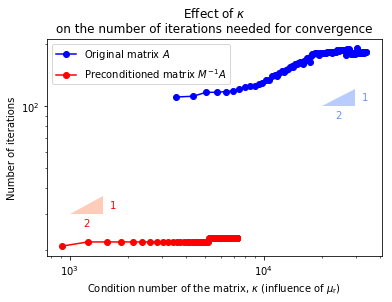
\includegraphics[width=\linewidth]{iter_cond.png}
		\caption{Évolution du nombre d'itérations en fonction de $\kappa$. Les triangles servent à visualiser la borne supérieure sur la pente.}
		\label{fig:iter_cond}
	\end{subfigure}\hfill
	\begin{subfigure}[t]{0.28\textwidth}
		\centering
		%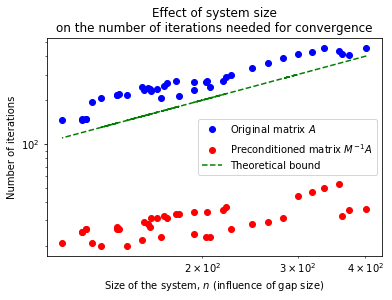
\includegraphics[width=\linewidth]{iter_n.png}
		\caption{Évolution du nombre d'itérations en fonction de la taille du système, en jouant sur la largeur de l'entrefer.}
		\label{fig:iter_n}
	\end{subfigure}\hfill
	\begin{subfigure}[t]{0.28\textwidth}
		\centering
		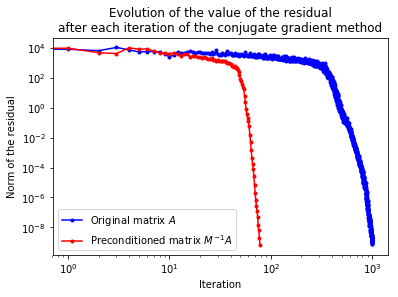
\includegraphics[width=\linewidth]{res_iter.png}
		\caption{Évolution de la norme du résidu à l'itération courante.}
		\label{fig:res_iter}
	\end{subfigure}
	\caption{Différents graphes pertinents pour l'analyse de convergence en section~\ref{sec:conv}.}
	\label{fig:conv_anal}
\end{figure}

\section*{Conclusion}
Les systèmes (symétriques) définis positifs tels que ceux issus du modèle \texttt{ccore} se rencontrent très fréquemment dans le monde de la physique et de l'ingénierie. Grâce aux méthodes itératives comme celle des gradients conjugués (basée sur l'itération d'Arnoldi), il est possible de profiter des propriétés intéressantes de ces matrices afin de diminuer fortement le temps nécessaire pour résoudre un système linéaire les contenant.

En faisant ce devoir, il est devenu apparent que trouver un bon préconditionneur est primordial afin de pouvoir espérer une convergence en peu d'itérations (mais qui ne soit pas trop difficile à calculer), mais que choisir celui-ci n'est pas aussi simple que cela n'en a l'air. Le préconditionneur \texttt{ILU0} semble donner un bon compromis entre facilité de calcul et diminution du nombre d'itérations.
\end{document}